\section*{Resultados e Discussões}

A implementação atestou a capacidade arquitetural em lidar com cargas massivas sob rígidas restrições de latência. Considerando o território nacional, o banco de dados processou 3.335.198 registros na tabela fato. A avaliação empírica revelou que a solução sustenta consultas pesadas com vazão superior a 2 requisições por segundo (\textit{QPS}) sem apresentar falhas de conexão (0\%) sob alta demanda analítica.

O sistema fornece Indicadores Chave de Desempenho (KPIs) sub-segundo, contabilizando a área consumida e perdas estimadas. A espacialização interativa em Minas Gerais (Fig. 1) mapeia a abrangência dos riscos e a proximidade geométrica das manchas ativas com infraestruturas vitais, terras indígenas e redes elétricas, permitindo a análise contínua da evolução dos incêndios.

\begin{figure}[H]
    \centering
    \caption{Mapa Analítico de Dispersão dos Focos no Território Mineiro}
    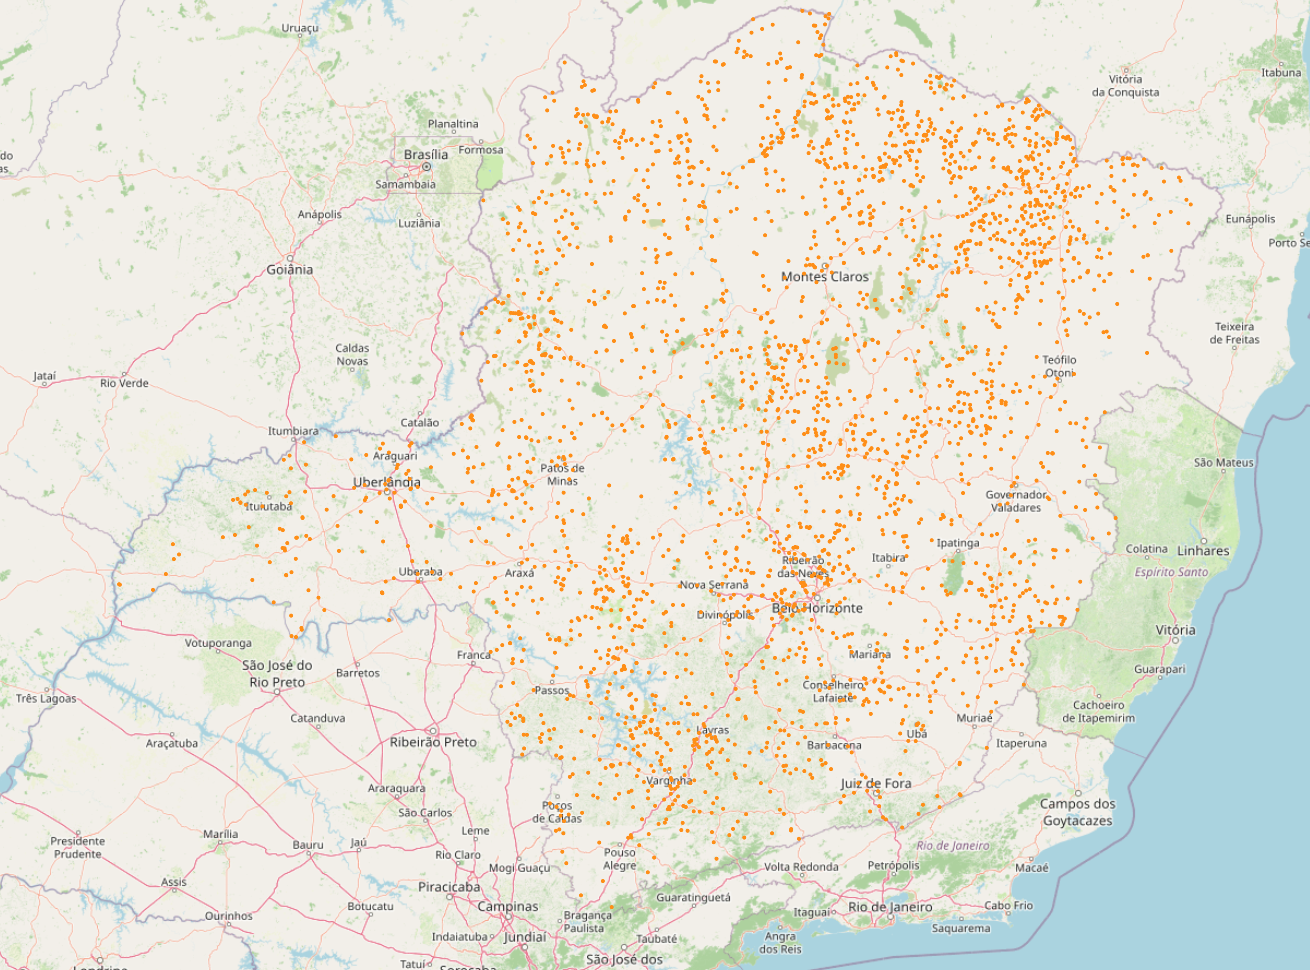
\includegraphics[width=0.7\textwidth]{MapaDeMInas.png}
    \fonte{Autores da pesquisa.}
    \label{fig:mapa}
\end{figure}

Para embasar a robustez, submeteu-se o motor a testes de estresse locais (8 CPUs, 7,5 GiB RAM), variando recursos dos contêineres de consulta (Broker e Historical). A Figura 2 detalha a vazão (QPS) pela concorrência. O perfil de maior alocação sustenta a vazão acima de 2 QPS até concorrência 4. Perfis restritos entram em saturação rapidamente, ratificando a importância do dimensionamento adequado da camada OLAP.

\begin{figure}[H]
    \centering
    \caption{Vazão Analítica do Sistema (QPS) em Função da Concorrência}
    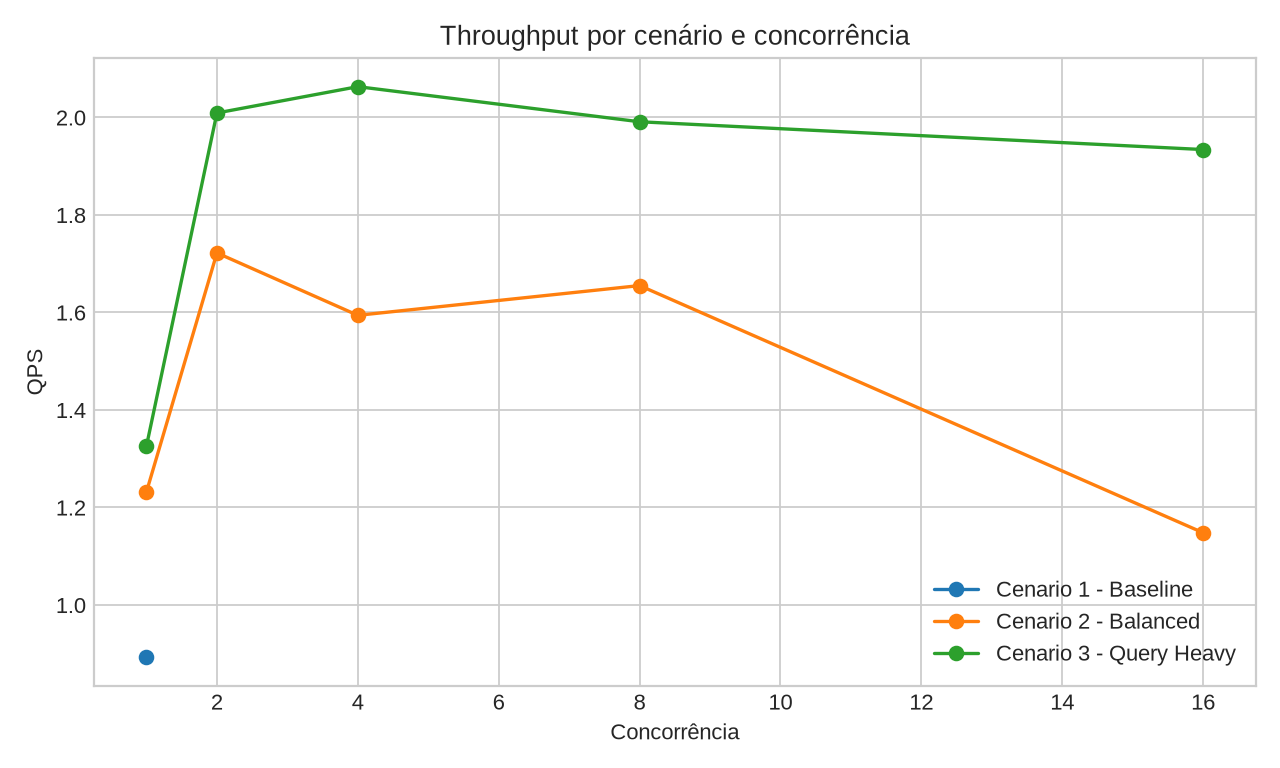
\includegraphics[width=0.9\textwidth]{qps_por_concorrencia.png}
    \fonte{Autores da pesquisa.}
    \label{fig:qps}
\end{figure}

Os resultados comprovam a exequibilidade de transformar registros isolados em inteligência ambiental rápida e coerente. A orquestração garante o cruzamento perene das ameaças contra alvos vulneráveis em tempo hábil para a Defesa Civil.
